% LaTeX figure snippets for main.tex
% These reference PDFs in the figures/ directory.

\begin{figure}[tbp]
\centering

\includegraphics[width=0.75\textwidth]{figures/fig_schematic.pdf}
\caption{\textbf{Thalamocortical loop architecture.} A recurrent cortical
network of $N = 256$ neurons is reciprocally connected to an uncoupled
thalamic population of $M = 32$ neurons via corticothalamic ($W_{TC}$) and
thalamocortical ($W_{CT}$) weights. Recurrent cortical connections
($W_{CC}$) are fixed. The local RFLO plasticity rule updates
thalamocortical weights $W_{CT}$; corticothalamic weights $W_{TC}$ are
either optimized by meta-learning on a slow timescale or set to an
idealized structure aligned with a specific cortical subspace.}
\label{fig:schematic}
\end{figure}

\begin{figure}[tbp]
\centering
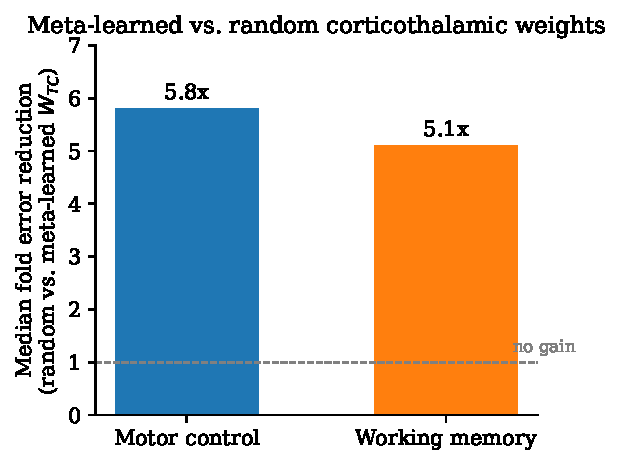
\includegraphics[width=0.62\textwidth]{figures/fig_metalearning_gain.pdf}
\caption{\textbf{Meta-learning reduces task error several fold relative to
random corticothalamic weights.} Median factor by which task performance
error decreases when $W_{TC}$ is meta-learned compared with the random
$W_{TC}$ baseline. Across simulations, meta-learning yields a 5.8-fold
improvement for the autonomous motor control task and a 5.1-fold
improvement for the working memory task. All models have $N = 256$
cortical neurons and $M = 32$ thalamic neurons; the dashed line marks the
level of no improvement.}
\label{fig:meta_gain}
\end{figure}

\begin{figure}[tbp]
\centering
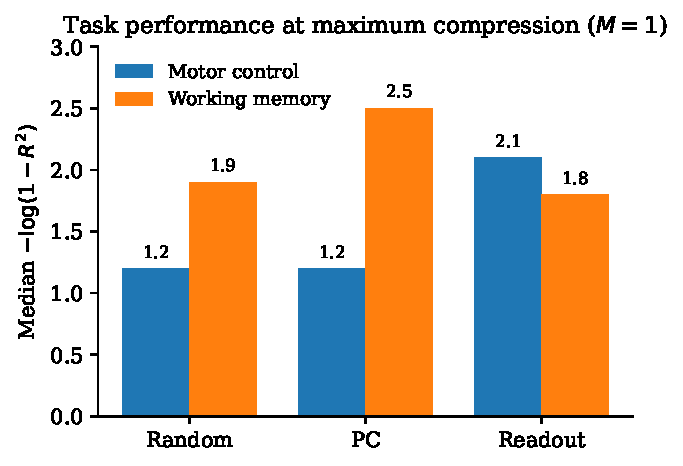
\includegraphics[width=0.72\textwidth]{figures/fig_idealized_m1.pdf}
\caption{\textbf{Idealized corticothalamic connectivity at maximum
compression.} Median $-\log(1 - R^2)$ for models with $M = 1$ and
corticothalamic weights aligned with a random direction, with the leading
principal component direction (PC), or with the readout direction. Higher
values indicate better performance. The autonomous motor control task is
optimally supported by readout-aligned corticothalamic weights (2.1), while
the working memory task is optimally supported by PC-aligned weights (2.5).
Random connectivity learns poorly in both tasks (1.2 and 1.9).}
\label{fig:idealized_m1}
\end{figure}

\begin{figure}[tbp]
\centering
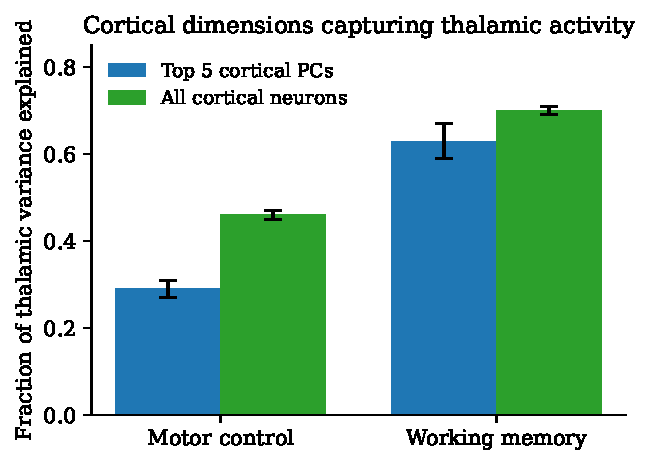
\includegraphics[width=0.72\textwidth]{figures/fig_thalamic_variance.pdf}
\caption{\textbf{Cortical dimensions capturing thalamic activity in mice.}
Fraction of variance in individual thalamic neurons explained by the top 5
cortical principal components versus by the full cortical population. The
top 5 cortical PCs capture 0.29 $\pm$ 0.02 of explainable thalamic
variance in motor control but 0.63 $\pm$ 0.04 in working memory,
consistent with the model prediction that motor thalamus is driven by
lower-variance readout-aligned directions while frontal thalamus is
driven by the leading principal components of cortical activity. Error
bars are $\pm 1$ SEM.}
\label{fig:thalamic_variance}
\end{figure}

\begin{figure}[tbp]
\centering
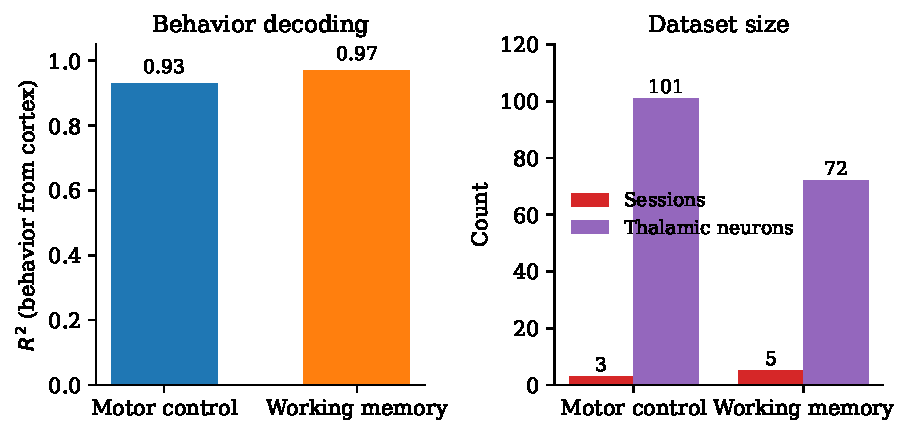
\includegraphics[width=0.85\textwidth]{figures/fig_behavior_decoding.pdf}
\caption{\textbf{Behavior decoding and dataset size for the two
re-analyzed neural recordings.} Left: Fraction of variance in behavior
(hand acceleration for motor control; choice for working memory)
explained by a linear readout of cortical population activity. Cortical
activity explains 0.93 of behavioral variance in motor control and 0.97
in working memory. Right: Number of recording sessions and number of
thalamic neurons in each dataset. Motor control: 3 sessions, 101
thalamic neurons (motor cortex and motor thalamus). Working memory: 5
sessions, 72 thalamic neurons (ALM and VM/VAL thalamus).}
\label{fig:behavior_decoding}
\end{figure}
